\documentclass[a4paper,12pt]{article}

% Основные пакеты
\usepackage[utf8]{inputenc}             % Поддержка кодировки UTF-8
\usepackage[T1, T2A]{fontenc}           % Поддержка кириллицы
\usepackage[english, russian]{babel}    % Поддержка русского и английского языков
\usepackage{graphicx}                   % Для вставки изображений
\usepackage{import}                     % Для продвинутого импорта (например, из Inkscape)
\usepackage{subcaption}                 % Для создания подписей к изображениям в сетке
\usepackage{float}                      % Для улучшенного размещения изображений
\usepackage{geometry}                   % Для управления отступами на странице
\usepackage{amsmath, amssymb, amsfonts} % Для математических формул и символов
\usepackage{booktabs}                   % Для красивых таблиц
\usepackage[dvipsnames]{xcolor}         % Для расширенной поддержки цветов
\usepackage[colorlinks]{hyperref}       % Для создания гиперссылок
\usepackage{indentfirst}                % Для красной строки в первом абзаце
\usepackage{listings}                   % Для оформления листингов кода
\usepackage{longtable}                  % Для длинных таблиц
\usepackage{makecell}                   % Для улучшенного форматирования ячеек таблиц
\usepackage{multirow}                   % Для объединения строк в таблицах
\usepackage{tabularray}                 % Для продвинутых таблиц
\usepackage{varwidth}                   % Для переменной ширины блоков
\usepackage{bm}                         % Для жирных математических символов
\usepackage{pifont}                     % Для специальных символов (например, галочек)
\usepackage{fontawesome}                % Для иконок

% Настройка отступов на странице
\geometry{left=2cm, right=2cm, bottom=2cm, top=2cm}

% Настройка гиперссылок
\hypersetup{
    linkcolor=blue,
    filecolor=magenta,
    urlcolor=cyan
}

% Настройка листингов
\definecolor{codegreen}{rgb}{0,0.6,0}
\definecolor{codegray}{rgb}{0.5,0.5,0.5}
\definecolor{codepurple}{rgb}{0.58,0,0.82}
\definecolor{backcolour}{rgb}{0.95,0.95,0.92}

\lstdefinestyle{codestyle}{
    backgroundcolor=\color{backcolour},
    commentstyle=\color{codegreen},
    keywordstyle=\color{blue},
    numberstyle=\tiny\color{codegray},
    stringstyle=\color{magenta},
    basicstyle=\ttfamily\footnotesize,
    breakatwhitespace=false,
    breaklines=true,
    captionpos=b,
    keepspaces=true,
    numbers=left,
    numbersep=5pt,
    showspaces=false,
    showstringspaces=false,
    showtabs=false,
    tabsize=2
}

\lstset{style=codestyle, extendedchars=\true}

% Путь к изображениям
\graphicspath{ {./images/} }

\begin{document}
\begin{titlepage}
    \centering
    \vspace*{1cm}

    {\large Министерство науки и высшего образования Российской Федерации}\\
    {\large ФЕДЕРАЛЬНОЕ ГОСУДАРСТВЕННОЕ АВТОНОМНОЕ ОБРАЗОВАТЕЛЬНОЕ УЧРЕЖДЕНИЕ ВЫСШЕГО ОБРАЗОВАНИЯ «НАЦИОНАЛЬНЫЙ ИССЛЕДОВАТЕЛЬСКИЙ УНИВЕРСИТЕТ ИТМО»}\\
    {\large (УНИВЕРСИТЕТ ИТМО)}\\

    \vspace{2cm}

    {\large Факультет «Систем управления и робототехники»}\\

    \vspace{3cm}

    \textbf{{\Huge ОТЧЕТ}\\
    {\Huge О ЛАБОРАТОРНОЙ РАБОТЕ №2}}\\

    \vspace{1cm}

    {\LARGE По дисциплине «Техническое зрение»}\\
    {\LARGE на тему: «Геометрические преобразования изображений»}\\

    \vspace{2cm}

    {\Large Студент:}\\
    Охрименко Ева ИСУ 409290\\

    \vspace{2cm}

    {\Large Проверил:}\\
    Шаветов Сергей Васильевич\\

    \vspace{4cm}

    {\large г. Санкт-Петербург}\\
    {\large 2025}

\end{titlepage}

\tableofcontents  % Оглавление
\newpage

\section{Цель работы}
Освоение основных видов отображений и использование геометрических преобразований для решения задач пространственной коррекции изображений.

\section{Task. Простейшие геометрические преобразования}
В этом задании рассмотрим несколько геометрических преобразований над следующей картинкой с котиком.

\begin{figure}[htbp]
    \centering
    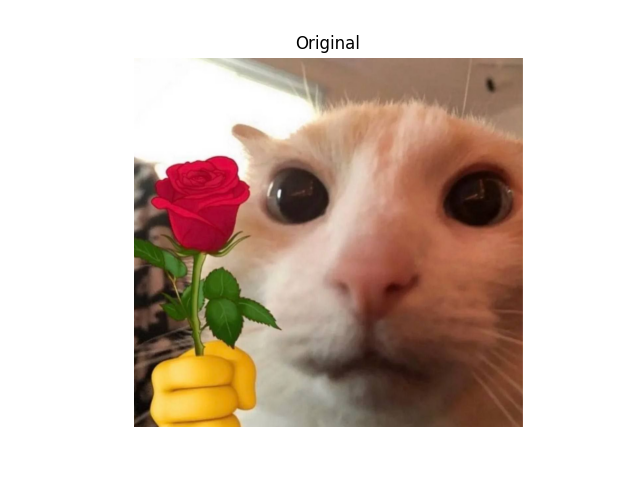
\includegraphics[width=0.8\textwidth]{lab2/task1/Figure_1.png}
    \caption{Оригинальное изображение}
    \label{fig:my_image}
\end{figure}

Также приведу функции, которые будут вложены в другие функции в ходе написания функций для преобразования. Они были написаны, потому что мне так было удобнее работать.

\begin{lstlisting}[language=Python, caption=Функции для удобства]
def show(image, title):
    plt.imshow(image)
    plt.title(title)
    plt.axis('off')
    plt.show()

def convert_to_rgb(image):
    return cv2.cvtColor(image, cv2.COLOR_BGR2RGB)

def size(image):
    rows, cols = image.shape[0:2]
    return rows, cols
\end{lstlisting}

А также приведу основной код программы, который загружает исходное изображение, применяет функции (из моего модуля \texttt{defs}) и выводит геометрические преобразования с использованием лямбда выражений.

\begin{lstlisting}[language=Python, caption=main]
import cv2
import matplotlib.pyplot as plt
from defs import *
import os

image_path = os.path.join(os.path.dirname(__file__), "image.jpg")
I1 = cv2.imread(image_path)

I = cv2.imread(image_path)
I_rgb = convert_to_rgb(I)

operations = [
    ("Original", lambda img: img),
    ("Shifted", lambda img: sdvig(img, 50, 100)),
    ("Reflected by OX", lambda img: reflectOX(img)),
    ("Reflected by OY", lambda img: reflectOY(img)),
    ("Scaled", lambda img: scaling(img, 1.7, 0.5)),
    ("Rotated", lambda img: rotate(img, 30)),
    ("Affined", lambda img: affine_transform(img, 
        np.float32([[50, 300], [150, 200], [50, 50]]), 
        np.float32([[50, 200], [250, 200], [50, 100]]))),
    ("Beveled", lambda img: bevel(img, 0.5)),
    ("piecewiselineared", lambda img: (piecewiselinear(img, 2))),
    ("projectived", lambda img: (projective(img, 1.1, 0.35, 0, 0.2, 1.1, 0, 0.00075, 0.00005, 1))),
    ("polynomialed", lambda img: (polynomial(img, np.array([[0, 0], [1, 0], [0, 1], [0.0001, 0], [0.002, 0], [0.001, 0]])))),
    ("sinusoidaled", lambda img: (sinusoidal(img, 20, 90)))
]
for title, operation in operations:
    result = operation(I)
    result_rgb = convert_to_rgb(result)
    show(result_rgb, title)
\end{lstlisting}

\subsection{Сдвиг}

Матрица преобразования \( T \) задается как:

\[
T = \begin{bmatrix}
1 & 0 & t_x \\
0 & 1 & t_y \\
\end{bmatrix}.
\]

Новые координаты пикселя \( (x', y') \) вычисляются по формуле:

\[
\begin{bmatrix}
x' \\
y' \\
\end{bmatrix}
= T \cdot
\begin{bmatrix}
x \\
y \\
1 \\
\end{bmatrix}
=
\begin{bmatrix}
x + t_x \\
y + t_y \\
\end{bmatrix}.
\]

\begin{lstlisting}[language=Python, caption=Функция сдвига изображения]
def sdvig(image, tx, ty):
    rows, cols = size(image)
    T = np.float32([[1, 0, tx], [0, 1, ty]])
    shifted_image = cv2.warpAffine(image, T, (cols, rows))
    return shifted_image
\end{lstlisting}

В моем коде \( t_x = 50 \) и \( t_y = 100 \). То есть картинка сдвинется вправо на 50 пикселей и на 100 пикселей вниз. Этот успех можно наблюдать на следующей картинке.

\begin{figure}[H]
    \centering
    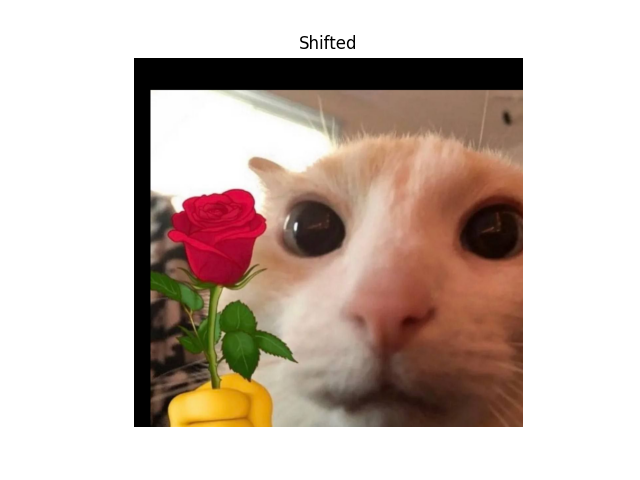
\includegraphics[width=0.8\textwidth]{lab2/task1/Figure_2.png}
    \caption{Сдвинутое изображение}
    \label{fig:shifted_image}
\end{figure}

\subsection{Отражение относительно осей \( OX \) и \( OY \)}

Матрица преобразования для отражения относительно оси \( OX \) задается как:

\[
T_{\text{OX}} = \begin{bmatrix}
1 & 0 & 0 \\
0 & -1 & \text{rows} - 1 \\
\end{bmatrix},
\]

где \(\text{rows}\) — высота изображения. Тогда новые координаты \( \begin{bmatrix} x' \\ y' \end{bmatrix} \) вычисляются как:

\[
\begin{bmatrix}
x' \\
y' \\
\end{bmatrix}
= \begin{bmatrix}
1 & 0 & 0 \\
0 & -1 & \text{rows} - 1 \\
\end{bmatrix} \cdot
\begin{bmatrix}
x \\
y \\
1 \\
\end{bmatrix}
=
\begin{bmatrix}
x \\
\text{rows} - 1 - y \\
\end{bmatrix}.
\]

Матрица преобразования для отражения относительно оси \( OY \) задается как:

\[
T_{\text{OY}} = \begin{bmatrix}
-1 & 0 & \text{cols} - 1 \\
0 & 1 & 0 \\
\end{bmatrix},
\]

где \(\text{cols}\) — ширина изображения. Тогда новые координаты \( \begin{bmatrix} x' \\ y' \end{bmatrix} \) вычисляются как:

\[
\begin{bmatrix}
x' \\
y' \\
\end{bmatrix}
= \begin{bmatrix}
-1 & 0 & \text{cols} - 1 \\
0 & 1 & 0 \\
\end{bmatrix} \cdot
\begin{bmatrix}
x \\
y \\
1 \\
\end{bmatrix}
=
\begin{bmatrix}
\text{cols} - 1 - x \\
y \\
\end{bmatrix}.
\]

\begin{lstlisting}[language=Python, caption=Функции отражения]
def reflectOX(image):
    rows, cols = size(image)
    T = np.float32([[1, 0, 0], [0, -1, rows - 1]])
    I_reflect = cv2.warpAffine(image, T, (cols, rows))
    return I_reflect

def reflectOY(image):
    rows, cols = size(image)
    T = np.float32([[-1, 0, cols - 1], [0, 1, 0]])
    I_reflect = cv2.warpAffine(image, T, (cols, rows))
    return I_reflect
\end{lstlisting}

А теперь посмотрим на успешный вывод двух отраженных котиков:

\begin{figure}[H]
    \centering
    \begin{minipage}{0.48\textwidth}
        \centering
        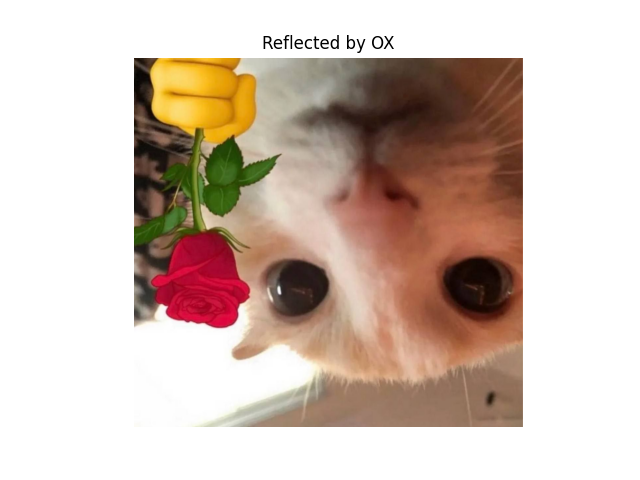
\includegraphics[width=\linewidth]{lab2/task1/Figure_3.png}
        \caption{Отражение относительно \( OX \)}
        \label{fig:reflect_ox}
    \end{minipage}
    \hfill
    \begin{minipage}{0.48\textwidth}
        \centering
        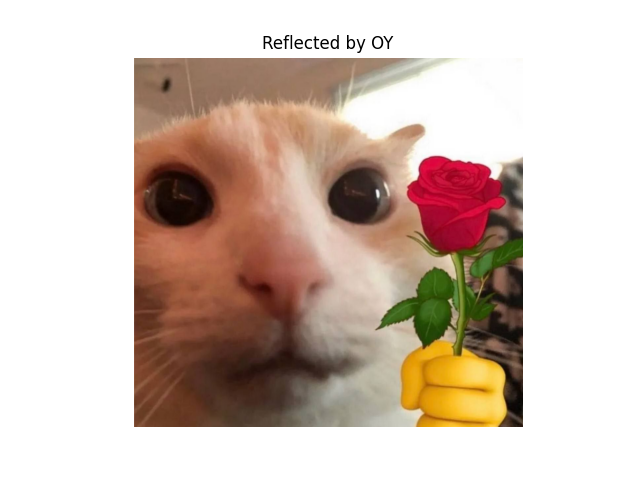
\includegraphics[width=\linewidth]{lab2/task1/Figure_4.png}
        \caption{Отражение относительно \( OY \)}
        \label{fig:reflect_oy}
    \end{minipage}
\end{figure}

\subsection{Однородное масштабирование}
Матрица преобразования для масштабирования задается как:

\[
T = \begin{bmatrix}
s_x & 0 & 0 \\
0 & s_y & 0 \\
\end{bmatrix},
\]

где \( s_x \) — коэффициент масштабирования по оси \( OX \), \( s_y \) — коэффициент масштабирования по оси \( OY \).

Новые координаты пикселя 
\begin{bmatrix}
x' \\
y' \\
\end{bmatrix} 
вычисляются по формуле:

\[
\begin{bmatrix}
x' \\
y' \\
\end{bmatrix}
= \begin{bmatrix}
s_x & 0 & 0 \\
0 & s_y & 0 \\
\end{bmatrix} \cdot
\begin{bmatrix}
x \\
y \\
1 \\
\end{bmatrix}
=
\begin{bmatrix}
s_x \cdot x \\
s_y \cdot y \\
\end{bmatrix}.
\]

\begin{lstlisting}[language=Python, caption=Функция масштабирования]
def scaling(image, scale_x, scale_y):
    rows, cols = size(image)
    T = np.float32([[scale_x, 0, 0] ,[0, scale_y, 0]])
    I_scale = cv2.warpAffine(image, T, (int(cols * scale_x), int(rows*scale_y)))
    return I_scale
\end{lstlisting}

В моем коде я использовала \( s_x = 1.7 \) и \( s_y = 0.5 \). То есть бедного котика сплющит. Посмотрим на вывод:

\begin{figure}[H]
    \centering
    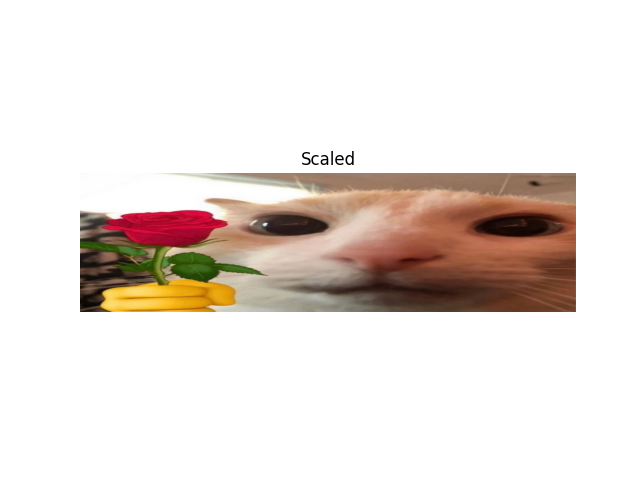
\includegraphics[width=0.8\textwidth]{lab2/task1/Figure_5.png}
    \caption{Однородное масштабирование}
    \label{fig:my_image}
\end{figure}

\subsection{Поворот}

Матрица преобразования для поворота на угол \( \phi \) задается как:

\[
T = \begin{bmatrix}
\cos(\phi) & -\sin(\phi) & 0 \\
\sin(\phi) & \cos(\phi) & 0 \\
\end{bmatrix},
\]

где: \( \phi \) — угол поворота в радианах

Новые координаты пикселя
\begin{bmatrix}
x' \\
y' \\
\end{bmatrix} 
вычисляются по формуле:

\[
\begin{bmatrix}
x' \\
y' \\
\end{bmatrix}
= \begin{bmatrix}
\cos(\phi) & -\sin(\phi) & 0 \\
\sin(\phi) & \cos(\phi) & 0 \\
\end{bmatrix} \cdot
\begin{bmatrix}
x \\
y \\
1 \\
\end{bmatrix}
=
\begin{bmatrix}
\cos(\phi) \cdot x - \sin(\phi) \cdot y \\
\sin(\phi) \cdot x + \cos(\phi) \cdot y \\
\end{bmatrix}.
\]


\begin{lstlisting}[language=Python, caption=Функция поворота]
def rotate(image, phi):
    rows, cols = size(image)
    phi = math.radians(phi)
    T = np.float32([[ math.cos(phi), -math.sin(phi), 0], [math.sin(phi), math.cos(phi), 0]])
    I_rotate = cv2.warpAffine(image, T, (cols, rows))
    return I_rotate
\end{lstlisting}

В моем коде \( \phi = 30^\circ \). То есть картинка повернется на \( 30^\circ \).


\begin{figure}[H]
    \centering
    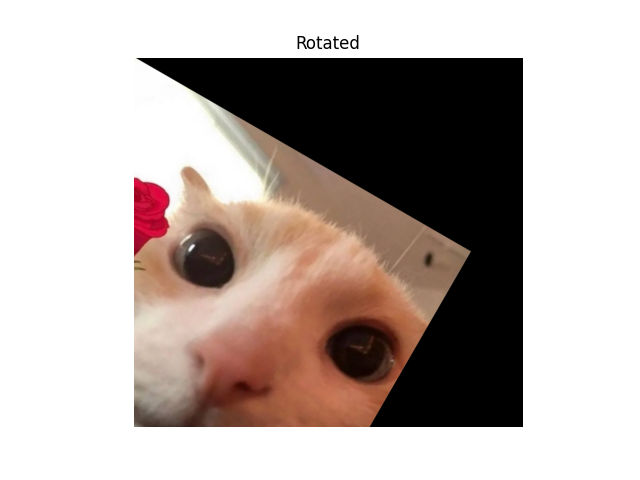
\includegraphics[width=0.8\textwidth]{lab2/task1/Figure_6.png}
    \caption{Поворот на \( 30^\circ \)}
    \label{fig:my_image}
\end{figure}

\subsection{Афинное отображение}
Матрица преобразования для аффинного преобразования задается как:
\[
T = \begin{bmatrix} 
a_{11} & a_{12} & b_1 \\ 
a_{21} & a_{22} & b_2 
\end{bmatrix},
\]

где \( a_{ij} \) — коэффициенты, задающие поворот, масштабирование и сдвиг, \( b_i \) — коэффициенты сдвига.


Новые координаты пикселя  \begin{bmatrix} x' \\ y' \end{bmatrix} вычисляются по формуле:

\[
\begin{bmatrix} x' \\ y' \end{bmatrix} = 
\begin{bmatrix} 
a_{11} & a_{12} & b_1 \\ 
a_{21} & a_{22} & b_2 
\end{bmatrix} 
\cdot 
\begin{bmatrix} x \\ y \\ 1 \end{bmatrix} 
= 
\begin{bmatrix} 
a_{11} \cdot x + a_{12} \cdot y + b_1 \\ 
a_{21} \cdot x + a_{22} \cdot y + b_2 
\end{bmatrix}.
\]

\begin{lstlisting}[language=Python, caption=Функция афинного отображения]
def affine_transform(image, pts_src, pts_dst):
    rows, cols = size(image)
    T = cv2.getAffineTransform(pts_src, pts_dst)
    affine_image = cv2.warpAffine(image, T, (cols, rows))
    return affine_image
\end{lstlisting}
Мое изображение будет повернуто, масштабировано и смещено в соответствии с заданными точками. Посмотрим на результат.

\begin{figure}[H]
    \centering
    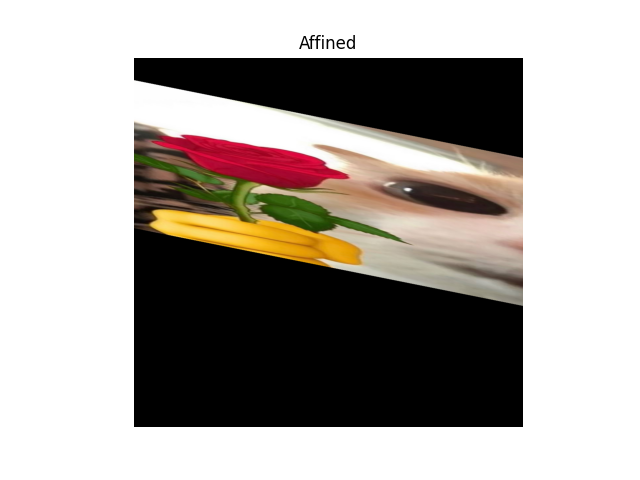
\includegraphics[width=0.8\textwidth]{lab2/task1/Figure_7.png}
    \caption{Афинное отображение}
    \label{fig:my_image}
\end{figure}

\subsection{Скос}
Матрица преобразования для скоса изображения задается как:

\[
T = \begin{bmatrix} 
1 & \text{skos} & 0 \\ 
0 & 1 & 0 
\end{bmatrix},
\]

где \(\text{skos}\) — коэффициент скоса по горизонтали.

Новые координаты пикселя  \begin{bmatrix} x' \\ y' \end{bmatrix} вычисляются по формуле:

\[
\begin{bmatrix} x' \\ y' \end{bmatrix} = 
\begin{bmatrix} 
1 & \text{skos} & 0 \\ 
0 & 1 & 0 
\end{bmatrix} 
\cdot 
\begin{bmatrix} x \\ y \\ 1 \end{bmatrix} 
= 
\begin{bmatrix} 
x + \text{skos} \cdot y \\ 
y 
\end{bmatrix}.
\]
\begin{lstlisting}[language=Python, caption=Функция скоса]
def affine_transform(image, pts_src, pts_dst):
    rows, cols = size(image)
    T = cv2.getAffineTransform(pts_src, pts_dst)
    affine_image = cv2.warpAffine(image, T, (cols, rows))
    return affine_image
\end{lstlisting}

Мое изображение будет скошено с коэффициентом \( skos = 0.5 \).

\begin{figure}[H]
    \centering
    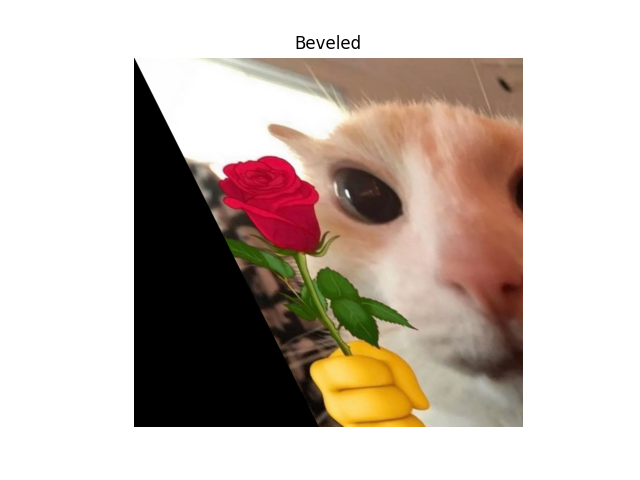
\includegraphics[width=0.8\textwidth]{lab2/task1/Figure_8.png}
    \caption{Скос}
    \label{fig:my_image}
\end{figure}

\subsection{Кусочно-линейное отображение}

Матрица преобразования для кусочно-линейного растяжения изображения задается как:

\[
T = \begin{bmatrix} 
\text{stretch} & 0 & 0 \\ 
0 & 1 & 0 
\end{bmatrix},
\]

где  \(\text{stretch}\) — коэффициент растяжения по горизонтали.

Новые координаты пикселя  \begin{bmatrix} x' \\ y' \end{bmatrix} вычисляются по формуле:

\[
\begin{bmatrix} x' \\ y' \end{bmatrix} = 
\begin{bmatrix} 
\text{stretch} & 0 & 0 \\ 
0 & 1 & 0 
\end{bmatrix} 
\cdot 
\begin{bmatrix} x \\ y \\ 1 \end{bmatrix} 
= 
\begin{bmatrix} 
\text{stretch} \cdot x \\ 
y 
\end{bmatrix}.
\]

\begin{lstlisting}[language=Python, caption=Функция кусочно-линейного отображения]
def piecewiselinear(image, stretch):
    rows, cols = size(image)
    T = np.float32([[stretch, 0, 0], [0, 1, 0]])
    I_piecewiselinear = image.copy()
    I_piecewiselinear[:, int(cols/2):, :] = cv2.warpAffine(I_piecewiselinear[:, int(cols/2):, :], T, (cols - int(cols/2), rows))
    return I_piecewiselinear
\end{lstlisting}

В моем коде \( strech = 2 \). Правая часть картинки будет растянута с этим коэффициентом.

\begin{figure}[H]
    \centering
    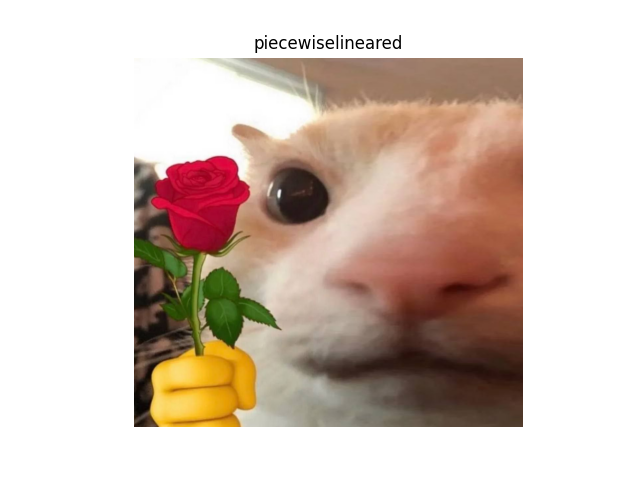
\includegraphics[width=0.8\textwidth]{lab2/task1/Figure_9.png}
    \caption{Кусочно-линейное отображение}
    \label{fig:my_image}
\end{figure}

\subsection{Проекционное отображение}

Матрица преобразования для пр преобразования задается как:

\[
T = \begin{bmatrix} 
a & b & c \\ 
d & e & f \\ 
g & h & i 
\end{bmatrix},
\]

где \(a, b, c, d, e, f, g, h, i\) — коэффициенты, задающие проекционное преобразование.

Новые координаты пикселя  \begin{bmatrix} x' \\ y' \end{bmatrix} вычисляются по формуле:

\[
\begin{bmatrix} x' \\ y' \end{bmatrix} = 
\begin{bmatrix} 
\frac{a \cdot x + b \cdot y + c}{g \cdot x + h \cdot y + i} \\ 
\frac{d \cdot x + e \cdot y + f}{g \cdot x + h \cdot y + i} 
\end{bmatrix}.
\]

\begin{lstlisting}[language=Python, caption=Функция проекционного отображения]
def piecewiselinear(image, stretch):
    rows, cols = size(image)
    T = np.float32([[stretch, 0, 0], [0, 1, 0]])
    I_piecewiselinear = image.copy()
    I_piecewiselinear[:, int(cols/2):, :] = cv2.warpAffine(I_piecewiselinear[:, int(cols/2):, :], T, (cols - int(cols/2), rows))
    return I_piecewiselinear
\end{lstlisting}

В моем коде коэффициенты заданы так: \(a = 1.1, b = 0.35, c = 0, d = 0.2, e = 1.1, f = 0, g = 0.00075, h = 0.00005, i = 1\). Посмотрим на результат:

\begin{figure}[H]
    \centering
    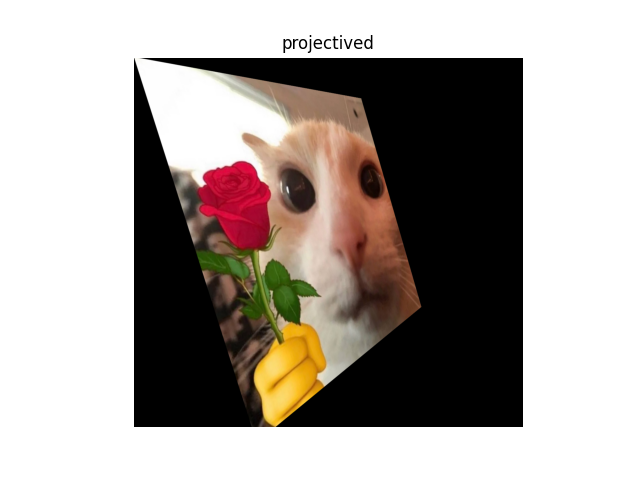
\includegraphics[width=0.8\textwidth]{lab2/task1/Figure_10.png}
    \caption{Проекционное отображение}
    \label{fig:my_image}
\end{figure}

\subsection{Полиномиальное отображение}

Матрица преобразования для полиномиального преобразования задается как:

\[
T = \begin{bmatrix} 
T_{0,0} & T_{0,1} \\ 
T_{1,0} & T_{1,1} \\ 
T_{2,0} & T_{2,1} \\ 
T_{3,0} & T_{3,1} \\ 
T_{4,0} & T_{4,1} \\ 
T_{5,0} & T_{5,1} 
\end{bmatrix},
\]

где  \(T_{i,j}\) — коэффициенты, задающие полиномиальное преобразование.

Новые координаты пикселя \begin{bmatrix} \( x' \) \\ \( y' \) \end{bmatrix} вычисляются по формуле:

\[
\begin{bmatrix}
\( x' \) \\ \( y' \)
\end{bmatrix}
=
\begin{bmatrix}
T_{0,0} & T_{1,0} & T_{2,0} & T_{3,0} & T_{4,0} & T_{5,0} \\
T_{0,1} & T_{1,1} & T_{2,1} & T_{3,1} & T_{4,1} & T_{5,1}
\end{bmatrix}
\cdot
\begin{bmatrix}
1 \\
x \\
y \\
x^2 \\
x \cdot y \\
y^2
\end{bmatrix} =
\]  
\[
= \begin{bmatrix}
T_{0,0} \cdot 1 + T_{1,0} \cdot x + T_{2,0} \cdot y + T_{3,0} \cdot x^2 + T_{4,0} \cdot x \cdot y + T_{5,0} \cdot y^2 \\
T_{0,1} \cdot 1 + T_{1,1} \cdot x + T_{2,1} \cdot y + T_{3,1} \cdot x^2 + T_{4,1} \cdot x \cdot y + T_{5,1} \cdot y^2
\end{bmatrix}.
\]

\begin{lstlisting}[language=Python, caption=Функция полиномиального отображения]
def polynomial(image, T):
    rows, cols = size(image)
    I_polynomial = np.zeros_like(image)
    x, y = np.meshgrid(np.arange(cols), np.arange(rows))
    xnew = np.round(T[0, 0] + x*T[1, 0] + y*T[2, 0] + x*x*T[3, 0] + x*y*T[4, 0] + y*y*T[5, 0]).astype(np.float32)
    ynew = np.round(T[0, 1] + x*T[1, 1] + y*T[2, 1] + x*x*T[3, 1] + x*y*T[4, 1] + y*y*T[5, 1]).astype(np.float32)
    mask = np.logical_and(np.logical_and(xnew >= 0, xnew < cols), np.logical_and(ynew >= 0, ynew < rows))
    if image.ndim == 2:
        I_polynomial[ynew[mask].astype(int), xnew[mask].astype(int)] = image[y[mask], x[mask]]
    else:
        I_polynomial[ynew[mask].astype(int), xnew[mask].astype(int), :] = image[y[mask], x[mask], :]
    return I_polynomial
\end{lstlisting}

Я подаю на вход такой массив коэффициентов
\[
\begin{bmatrix}
[0, 0], & [1, 0], & [0, 1], & [0.0001, 0], & [0.002, 0], & [0.001, 0]
\end{bmatrix}.
\] Посмотрим, как исказится изображение

\begin{figure}[H]
    \centering
    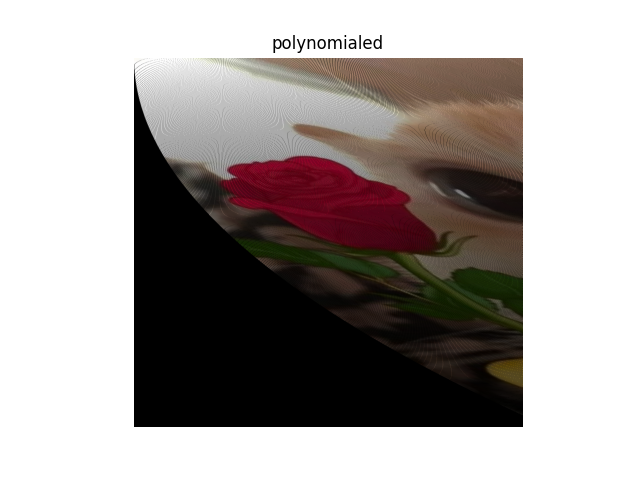
\includegraphics[width=0.8\textwidth]{lab2/task1/Figure_11.png}
    \caption{Полиномиальное отображение}
    \label{fig:my_image}
\end{figure}

\subsection{Синусоидальное отображение}


Новые координаты пикселя \((u, v)\) вычисляются по формуле:

\[
u = x + A \cdot \sin\left(\frac{2 \pi y}{f}\right),
\]
\[
v = y,
\]

где:
\begin{itemize}
    \item \(x\) и \(y\) — исходные координаты пикселя,
    \item \(A\) — амплитуда синусоидального искажения,
    \item \(f\) — частота синусоидального искажения.
\end{itemize}



\begin{lstlisting}[language=Python, caption=Функция синусоидального отображения]
def polynomial(image, T):
    rows, cols = size(image)
    I_polynomial = np.zeros_like(image)
    x, y = np.meshgrid(np.arange(cols), np.arange(rows))
    xnew = np.round(T[0, 0] + x*T[1, 0] + y*T[2, 0] + x*x*T[3, 0] + x*y*T[4, 0] + y*y*T[5, 0]).astype(np.float32)
    ynew = np.round(T[0, 1] + x*T[1, 1] + y*T[2, 1] + x*x*T[3, 1] + x*y*T[4, 1] + y*y*T[5, 1]).astype(np.float32)
    mask = np.logical_and(np.logical_and(xnew >= 0, xnew < cols), np.logical_and(ynew >= 0, ynew < rows))
    if image.ndim == 2:
        I_polynomial[ynew[mask].astype(int), xnew[mask].astype(int)] = image[y[mask], x[mask]]
    else:
        I_polynomial[ynew[mask].astype(int), xnew[mask].astype(int), :] = image[y[mask], x[mask], :]
    return I_polynomial
\end{lstlisting}

Я подам в функцию параметры \(a = 20\), \(f = 90\). Котик станет волновым котиком, мне это напомнило помехи на старом телевизоре.

\begin{figure}[H]
    \centering
    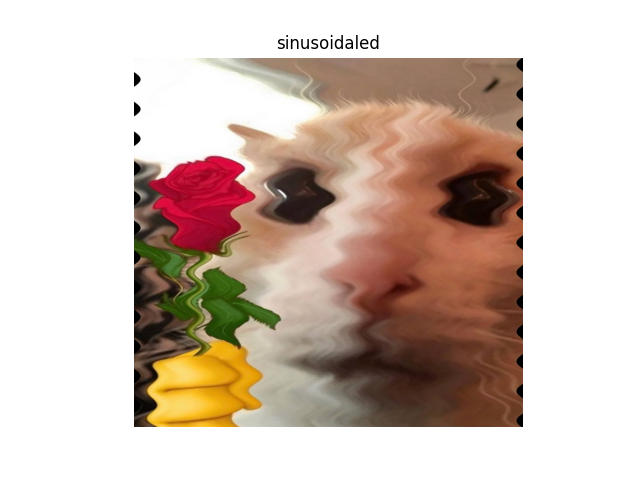
\includegraphics[width=0.8\textwidth]{lab2/task1/Figure_12.png}
    \caption{Синусоидальное отображение}
    \label{fig:my_image}
\end{figure}

\section{Task. Коррекция дистории}
Для этого задания выберу 2 искаженных изображения и попробую вернуть их к нормальному состоянию.

\begin{figure}[H]
    \centering
    \begin{minipage}{0.48\textwidth}
        \centering
        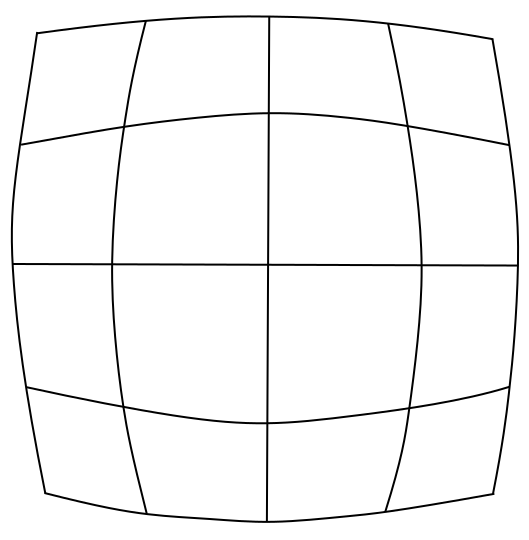
\includegraphics[width=\linewidth]{lab2/task2/bochka.png}
        \caption{Бочкообразная дистория}
        \label{fig:reflect_ox}
    \end{minipage}
    \hfill
    \begin{minipage}{0.48\textwidth}
        \centering
        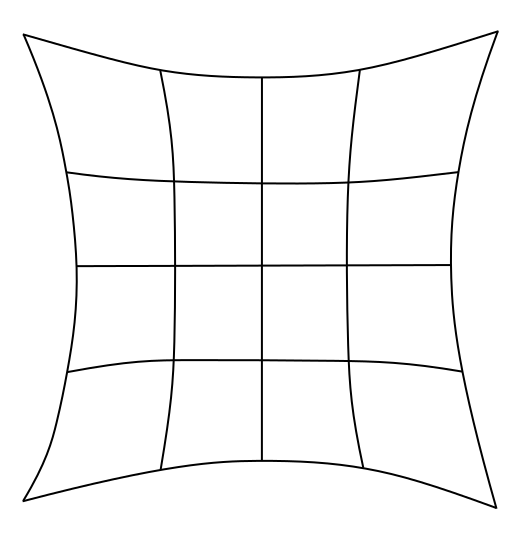
\includegraphics[width=\linewidth]{lab2/task2/podushka.png}
        \caption{Подушкообразная дистория}
        \label{fig:reflect_oy}
    \end{minipage}
\end{figure}

На изображениях нарисована сетка, которая была искажена двумя видами дистории.\\

Теперь приведу код, который загружает изображения и посылает их в функцию для коррекции дистории.

\begin{lstlisting}[language=Python, caption=main]
import cv2
import numpy as np
import matplotlib.pyplot as plt
from defs import *
import os

# Путь к файлу 1
image_path1 = os.path.join(os.path.dirname(__file__), "podushka.png")
I1 = cv2.imread(image_path1)
I_rgb_1 = convert_to_rgb(I1)

# Путь к файлу 2
image_path2 = os.path.join(os.path.dirname(__file__), "bochka.png")
I2 = cv2.imread(image_path2)
I_rgb_2 = convert_to_rgb(I2)

I_barrel = correct_distortion(I_rgb_1, 0.1, 0.12, "barrel")
I_pincushion = correct_distortion(I_rgb_2, 0.1, 0.12, "pincushion")

show(I_barrel, "Barrel Distortion Correction")
show(I_pincushion, "Pincushion Distortion Correction")
\end{lstlisting}

Теперь приступлю к написанию кода непосредственно для коррекции дисториий. Код для коррекции двух дисторий я решила записать в одну функцию. Для определения типа дистории используется передаваемый параметр \(type\).

\begin{lstlisting}[language=Python, caption=Коррекция дисторий]
def correct_distortion(image, F3, F5, type):
    rows, cols = size(image)
    xi, yi = np.meshgrid(np.arange(cols), np.arange(rows))
    xmid = cols / 2.0
    ymid = rows / 2.0
    xi = xi - xmid
    yi = yi - ymid
    r, theta = cv2.cartToPolar(xi / xmid, yi / ymid)
    if type == "barrel": r = r + F3 * r**3 + F5 * r**5  # Бочкообразная
    elif type == "pincushion": r = r - F3 * r**3 - F5 * r**5  # Подушкообразная
    else: raise ValueError("Используйте 'barrel' или 'pincushion'.")
    u, v = cv2.polarToCart(r, theta)
    u = u * xmid + xmid
    v = v * ymid + ymid
    corrected_image = cv2.remap(image, u.astype(np.float32), v.astype(np.float32), interpolation=cv2.INTER_LINEAR,)
    return corrected_image
\end{lstlisting}    

Что происходит в коде? Функция \texttt{correct\_distortion} корректирует искажения изображения по следующему алгоритму:

\begin{itemize}
    \item Создается сетка для всех пикселей
    \item Координаты центрируются относительно середины изображения
    \item Декартовы координаты преобразуются в полярные
    \item Радиус корректируется в зависимости от типа искажения
    \item  Полярные координаты преобразуются обратно в декартовы
    \item Координаты возвращаются к исходной системе
    \item Корректированное изображение создается с помощью \texttt{cv2.remap}
\end{itemize}

Тепреь применим функцию к нашим ранее заданным изображениям и оценим результат.

\begin{figure}[H]
    \centering
    \begin{minipage}{0.48\textwidth}
        \centering
        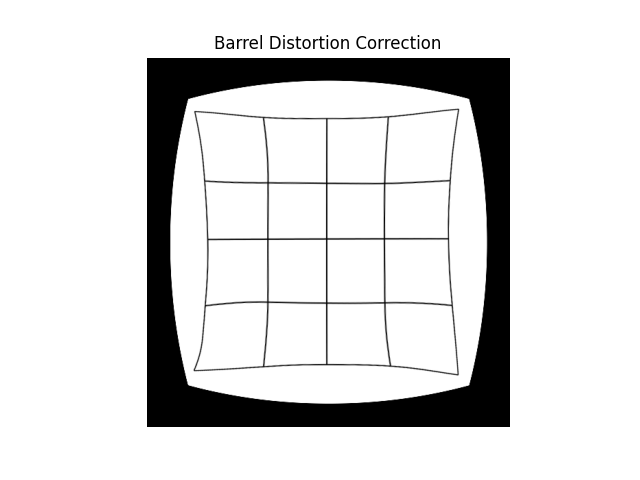
\includegraphics[width=\linewidth]{lab2/task2/Figure_1.png}
        \caption{Коррекция бочкообразной дистории}
        \label{fig:reflect_ox}
    \end{minipage}
    \hfill
    \begin{minipage}{0.48\textwidth}
        \centering
        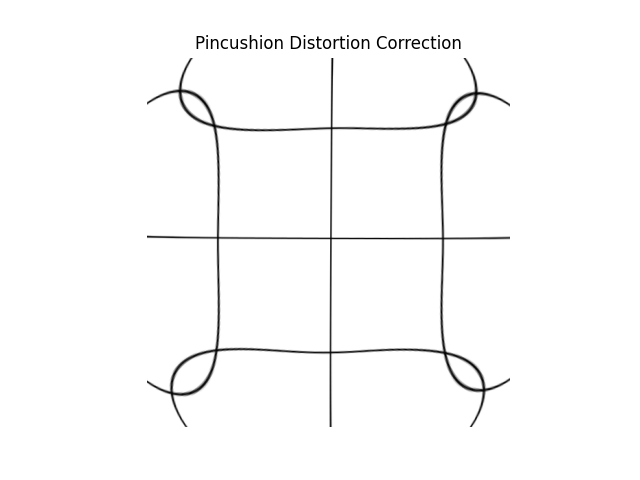
\includegraphics[width=\linewidth]{lab2/task2/Figure_2.png}
        \caption{Коррекция подушкообразной дистории}
        \label{fig:reflect_oy}
    \end{minipage}
\end{figure}
Могу сказать, что код помог и изображения с искажениями стали примерно похожи на изображения с квадратными сетками.

\section{Склейка изображений}
В этом задании мне нужно разрезать картинку так, чтобюы 2 разрезанные части имели общую площадь. А потом сшить эту картинку и посмотреть на результат. Для этого задания я взяла такие части одной картинки с улитками:

\begin{figure}[H]
    \centering
    \begin{minipage}{0.48\textwidth}
        \centering
        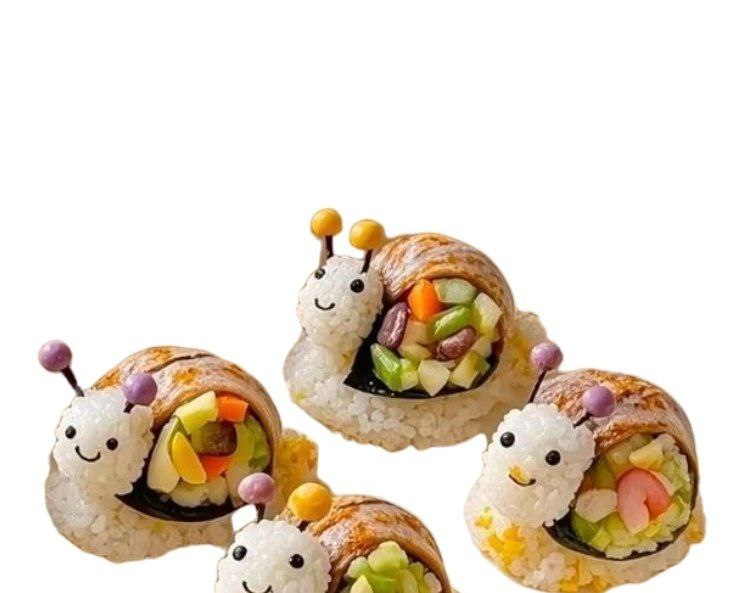
\includegraphics[width=\linewidth]{lab2/task3/ulitkiTop.jpg}
        \caption{Голова улиток}
        \label{fig:reflect_ox}
    \end{minipage}
    \hfill
    \begin{minipage}{0.48\textwidth}
        \centering
        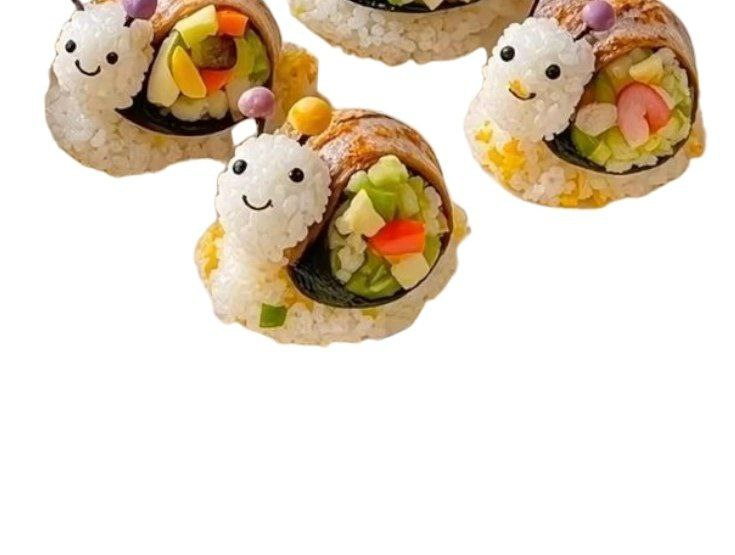
\includegraphics[width=\linewidth]{lab2/task3/ulitkiBottom.jpg}
        \caption{Панцырь улиток}
        \label{fig:reflect_oy}
    \end{minipage}
\end{figure}

Мои картинки соответствуют условию задания, можем приступить к написанию кода.


\begin{lstlisting}[language=Python, caption=Сшивка изображений]
import cv2
import os
import numpy as np

top_path = os.path.join(os.path.dirname(__file__), "ulitkiTop.jpg")
bot_path = os.path.join(os.path.dirname(__file__), "ulitkiBottom.jpg")
topPart = cv2.imread(top_path, cv2.IMREAD_COLOR)
botPart = cv2.imread(bot_path, cv2.IMREAD_COLOR)
templ_size = 10
templ = topPart[-templ_size:, :, :]
res = cv2.matchTemplate(botPart, templ, cv2.TM_CCOEFF)
min_val, max_val, min_loc, max_loc = cv2.minMaxLoc(res)
result_height = topPart.shape[0] + botPart.shape[0] - max_loc[1] - templ_size
result_width = topPart.shape[1]
result_channels = topPart.shape[2]
result_img = np.zeros((result_height, result_width, result_channels), dtype=np.uint8)
result_img[0:topPart.shape[0], :, :] = topPart
result_img[topPart.shape[0]:, :, :] = botPart[max_loc[1] + templ_size:, :, :]
cv2.imwrite("stitchedImage.jpg", result_img)
cv2.imshow("Stitched Image", result_img)
cv2.waitKey(0)
cv2.destroyAllWindows()
\end{lstlisting}    





Теперь посмотрим на вывод кода и сравним с исходным изображением сшитое.
\begin{figure}[H]
    \centering
    \begin{minipage}{0.48\textwidth}
        \centering
        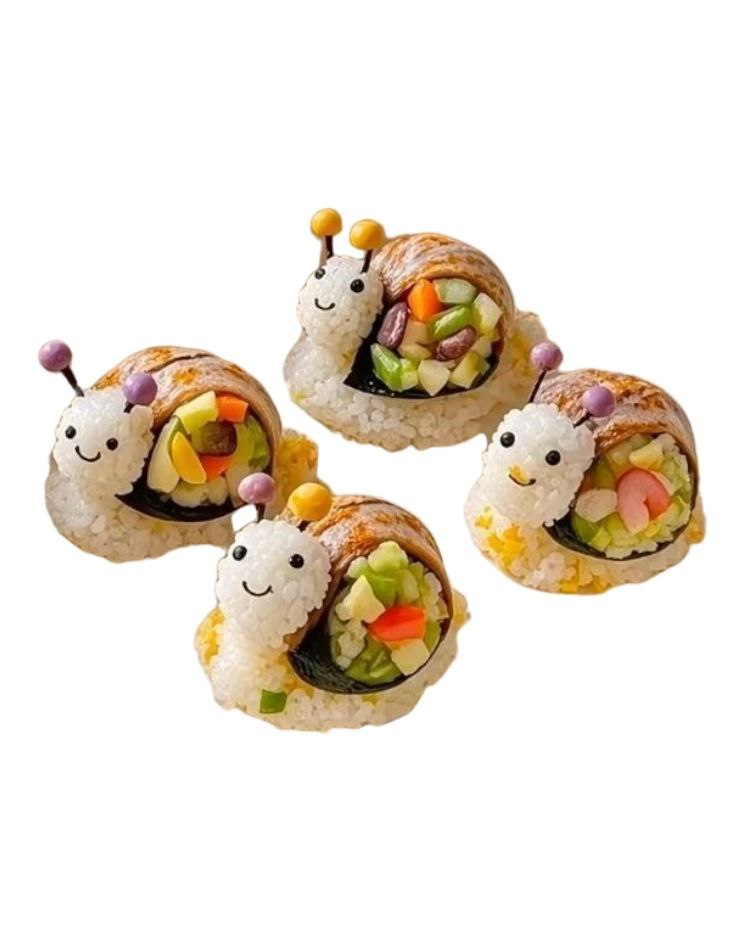
\includegraphics[width=\linewidth]{lab2/task3/orig.jpg}
        \caption{Оригинальное изображение}
        \label{fig:reflect_ox}
    \end{minipage}
    \hfill
    \begin{minipage}{0.48\textwidth}
        \centering
        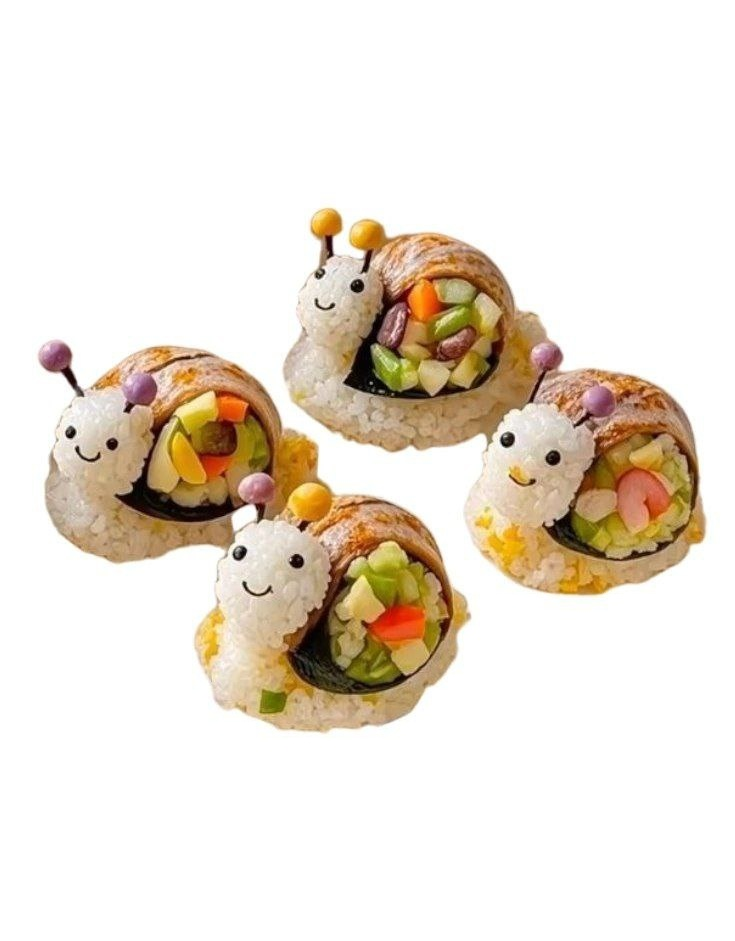
\includegraphics[width=\linewidth]{lab2/task3/stitchedImage.jpg}
        \caption{Сшитое изображение}
        \label{fig:reflect_oy}
    \end{minipage}
\end{figure}

Я не особо вижу разницу между картинками, задание успешно выполнено.


\section{Вывод}
В ходе выполнения работы я познакомилась с различными методами обработки изображений, начиная с простых преобразований, таких как повороты и масштабирование, и заканчивая более сложными операциями, включая коррекцию искажений и сшивание изображений. Также было приятно видеть несколько знакомых формул, поскольку что-то я изучала в курсе практической линейной алгебры. Репозиторий \href{https://github.com/decadeos/texViz/tree/main/lab2}{GitHub} с исходным кодом и tex-проектом.







\end{document}